\subsection{UC 16 - Modifica condivisione di un contatto} \label{sec:UC16}

    \begin{itemize}
        \item \textbf{Attore principale}: MUA;
        \item \textbf{Descrizione}: il MUA deve poter modificare una condivisione di un contatto nel sistema;
        \item \textbf{Precondizioni}: il MUA sta usando la funzionalità di modifica di una condivisione;
        \item \textbf{Postcondizioni}: il sistema modifica la condivisione del contatto con le informazioni fornite dal MUA;
        \item \textbf{Scenario principale}:
            \begin{enumerate}
                \item il MUA trasmette l'id del contatto di cui modificare la condivisione (\hyperref[sec:UC16.1]{UC 16.1});
                \item il MUA trasmette il nuovo indirizzo e-mail a cui condividere (\hyperref[sec:UC16.2]{UC 16.2});
                \item il sistema condivide il contatto;
            \end{enumerate}
        \item \textbf{Inclusioni}: nessuna;
        \item \textbf{Generalizzazioni}: nessuna;
        \item \textbf{Estensioni}: nessuna.
    \end{itemize}

    \begin{figure}[H]
        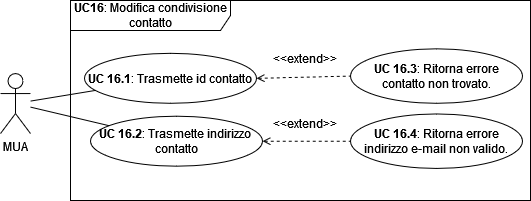
\includegraphics[width=0.85\textwidth]{sections/uc_imgs/UC16.png}
        \centering
        \caption{Diagramma sotto-casi UC 16}
    \end{figure}

    \subsubsection{UC 16.1 - Trasmette id contatto} \label{sec:UC16.1}
    \begin{itemize}
        \item \textbf{Attore principale}: MUA;
        \item \textbf{Descrizione}: il MUA trasmette l'id del contatto per modificarne la condivisione;
        \item \textbf{Precondizioni}: il MUA sta usando la funzionalità di modifica condivisione di un contatto;
        \item \textbf{Postcondizioni}: il sistema conosce l'id del contatto di cui modificare la condivisione;
        \item \textbf{Scenario principale}:
            \begin{enumerate}
                \item il MUA invia l'id del contatto per modificarne la condivisione;
            \end{enumerate}
        \item \textbf{Inclusioni}: nessuna;
        \item \textbf{Generalizzazioni}: nessuna;
        \item \textbf{Estensioni}:
            \begin{enumerate}[label=\alph*.]
                \item il sistema non riesce a modificare la condivisione del contatto perché l'id del contatto fornito non è stato trovato:
                \begin{enumerate}[label=\arabic*.]
                    \item il sistema ritorna un errore al MUA di contatto non trovato (\hyperref[sec:UC16.3]{UC 16.3}).
                \end{enumerate}
            \end{enumerate}
    \end{itemize}


    \subsubsection{UC 16.2 - Trasmette indirizzo contatto} \label{sec:UC16.2}
    \begin{itemize}
        \item \textbf{Attore principale}: MUA;
        \item \textbf{Descrizione}: il MUA trasmette il nuovo indirizzo e-mail per la condivisione al sistema;
        \item \textbf{Precondizioni}: il MUA sta usando la funzionalità di modifica condivisione di un contatto;
        \item \textbf{Postcondizioni}: il sistema conosce il nuovo indirizzo e-mail a cui condividere;
        \item \textbf{Scenario principale}:
            \begin{enumerate}
                \item il MUA invia il nuovo indirizzo e-mail per la condivisione al sistema;
                \item il sistema controlla che le informazioni ricevute rispettino il seguente requisito minimo:
                    \begin{itemize}
                        \item l'indirizzo e-mail del contatto non è una stringa vuota;
                    \end{itemize}
            \end{enumerate}
        \item \textbf{Inclusioni}: nessuna;
        \item \textbf{Generalizzazioni}: nessuna;
        \item \textbf{Estensioni}:
            \begin{enumerate}[label=\alph*.]
                \item il sistema non riesce a modificare la condivisione del contatto perché l'indirizzo e-mail fornito non è valido:
                \begin{enumerate}[label=\arabic*.]
                    \item il sistema ritorna un errore al MUA di indirizzo e-mail non valido (\hyperref[sec:UC16.4]{UC 16.4}).
                \end{enumerate}
            \end{enumerate}
    \end{itemize}


\subsubsection{UC 16.3 - Ritorna errore contatto non trovato} \label{sec:UC16.3}
    \begin{itemize}
        \item \textbf{Attore principale}: MUA;
        \item \textbf{Descrizione}: il sistema non riesce a modificare la condivisione del contatto perché il contatto non è stato trovato;
        \item \textbf{Precondizioni}: il MUA ha inviato l'id del contatto di cui modificare la condivisione;
        \item \textbf{Postcondizioni}: il sistema non modifica la condivisione del contatto, il MUA è stato notificato dell'errore;
        \item \textbf{Scenario principale}:
            \begin{enumerate}
                \item il sistema non trova il contatto con l'identificativo fornito dal MUA;
                \item il sistema non modifica la condivisione del contatto e notifica il MUA dell'errore;
            \end{enumerate}
        \item \textbf{Inclusioni}: nessuna;
        \item \textbf{Generalizzazioni}: nessuna;
        \item \textbf{Estensioni}: nessuna.
    \end{itemize}

    \subsubsection{UC 16.4 - Ritorna errore indirizzo e-mail non valido} \label{sec:UC16.4}
    \begin{itemize}
        \item \textbf{Attore principale}: MUA;
        \item \textbf{Descrizione}: il sistema non riesce a modificare la condivisione del contatto perché l'indirizzo e-mail fornito non rispetta i requisiti;
        \item \textbf{Precondizioni}: il MUA ha inviato il nuovo indirizzo e-mail a cui condividere;
        \item \textbf{Postcondizioni}: il sistema non modifica la condivisione del contatto, il MUA è stato notificato dell'errore;
        \item \textbf{Scenario principale}:
            \begin{enumerate}
                \item il sistema controlla la sintassi dell'indirizzo e-mail e trova un errore;
                \item il sistema non modifica la condivisione del contatto e notifica il MUA dell'errore;
            \end{enumerate}
        \item \textbf{Inclusioni}: nessuna;
        \item \textbf{Generalizzazioni}: nessuna;
        \item \textbf{Estensioni}: nessuna.
    \end{itemize}
